\documentclass[runningheads,a4paper]{llncs}

\usepackage{amssymb}
\setcounter{tocdepth}{3}
\usepackage{graphicx}

\usepackage{optidef}
\usepackage{balance}
\usepackage{amsmath}
\usepackage{helvet}
\usepackage{subfigure}
\usepackage{mdwmath}
\usepackage{mdwtab}
\usepackage{algorithm}
\usepackage{algpseudocode}
\usepackage{array}
\usepackage{multirow}
\usepackage{multicol}
\usepackage{natbib}

\usepackage{url}
\urldef{\mailsa}\path|{alfred.hofmann, ursula.barth, ingrid.haas, frank.holzwarth,|
\urldef{\mailsb}\path|anna.kramer, leonie.kunz, christine.reiss, nicole.sator,|
\urldef{\mailsc}\path|erika.siebert-cole, peter.strasser, lncs}@springer.com|    
\newcommand{\keywords}[1]{\par\addvspace\baselineskip
\noindent\keywordname\enspace\ignorespaces#1}

\algnewcommand\algorithmicInitial{\textbf{Initialize:}}
\algnewcommand\Initial{\item[\algorithmicInitial]}
\algnewcommand\algorithmicIterate{\textbf{Iterate:}}
\algnewcommand\Iterate{\item[\algorithmicIterate]}
\algnewcommand\algorithmicInput{\textbf{Input:}}
\algnewcommand\Input{\item[\algorithmicInput]}

\makeatletter
\def\@biblabel#1{#1.}
\makeatother

\begin{document}

\mainmatter  % start of an individual contribution

% first the title is needed
\title{Variance Reduced Stochastic Optimization for PCA and PLS}

% a short form should be given in case it is too long for the running head
%\titlerunning{Lecture Notes in Computer Science: Authors' Instructions}

% the name(s) of the author(s) follow(s) next
%
% NB: Chinese authors should write their first names(s) in front of
% their surnames. This ensures that the names appear correctly in
% the running heads and the author index.
%
\author{Erxue Min
\and Yawei Zhao\and Jun Long\and Jianping Yin
}
%
\authorrunning{Lecture Notes in Computer Science: Authors' Instructions}
% (feature abused for this document to repeat the title also on left hand pages)

% the affiliations are given next; don't give your e-mail address
% unless you accept that it will be published
\institute{College of Computer, National University of Defense Technology,\\
Changsha, China 410073\\
%\mailsa\\
%\mailsb\\
%\mailsc\\
%\url{http://www.springer.com/lncs}
}

%
% NB: a more complex sample for affiliations and the mapping to the
% corresponding authors can be found in the file "llncs.dem"
% (search for the string "\mainmatter" where a contribution starts).
% "llncs.dem" accompanies the document class "llncs.cls".
%

\toctitle{Lecture Notes in Computer Science}
\tocauthor{Authors' Instructions}
\maketitle


\begin{abstract}
%The abstract should summarize the contents of the paper and should contain at least 70 and at most 150 words. It should be written using the
Principal Component Analysis(PCA) is a dimensionality reduction technique which extracts the representative components of the data. Partial Least Squares(PLS) models the covariance structure between a pair of data matrices. The objective function of the two problems are similar and thus can often be solved by identical algorithms. Deterministic methods suffers from prohibitive computation cost in large-scale applications, while the stochastic algorithms fail to achieve high-accuracy solutions. In this paper, we propose stochastic optimization methods with variance reduction to solve PCA and PLS, which ensure to obtain high-accuracy solutions with enough computation cost and rapidly converge to an approximate optima with  few iterations. Extensive experiments demonstrate the significant performance of our method.
\keywords{PCA, PLS, SAGA}
\end{abstract}


\section{Introduction}
\label{introduction}
Principal component analysis (PCA) is a popular dimensionality reduction technique widely used in many areas, such as machine learning, statistics, computer vision \citep{Stockman2001Computer}. The goal of PCA is to find the maximal (uncentered) variance $k$-dimensional subspace with respect to a $d \times n$ matrix $X = (\mathbf{x}_1, ... , \mathbf{x}_n)$, where $\mathbf{x}_i \in \mathbb{R}^d$ with $i \in \{1,2, ... , n\}$. It is equivalent to solve the following optimization problem:
\begin{equation}
\label{pca-obj}
\begin{aligned}
& \underset{W}{\text{maximize}}
& & \mathrm{Trace}(W^{\top}(\frac{1}{n}\sum\limits_{i=1}^{n}\mathbf{x}_{i}{\mathbf{x}_i}^\top)W) \\
& \text{subject to}
& & W^{\top}W=I. \\
%&&& X \succeq 0.
\end{aligned}
\end{equation}
The  $d \times k$ matrix $W$ is used to parameterize the subspace.
Partial least squares (PLS) \citep{Chiang2001Partial}, a ubiquitous method for bilinear factor analysis, is widely used in information retrieval \citep{Salton2003Information} and machine learning. It solves the following problem: given a dataset of $n$ samples including  two sets of features, 
%$x \in \mathbb{R}^{d_x}$ and $y \in \mathbb{R}^{d_y}$, respectively, 
the $d_x \times n$ matrix $X = (\mathbf{x}_1, ... , \mathbf{x}_n)$ and the $d_y \times n$ matrix $Y = (\mathbf{y}_1, ... , \mathbf{y}_n)$, what is the $k$-dimensional subspace that captures most of the covariance between the two views. 
The PLS problem can be expressed as:
\begin{equation}
\label{pls-obj}
\begin{aligned}
& \underset{U,V}{\text{maximize}}
& & \mathrm{Trace}(U^{\top}(\frac{1}{n}\sum\limits_{i=1}^{n}\mathbf{x}_{i}{\mathbf{y}_i}^\top)V) \\
& \text{subject to}
& & U^{\top}U = I, V^{\top}V=I \\
%&&& X \succeq 0.
\end{aligned}
\end{equation}
The pair of  matrices $U \in \mathbb{R}^{d_x \times k}$ and $V \in \mathbb{R}^{d_y \times k}$ are the solution of PLS. 
It is obvious that the objective functions of PCA and PLS are quite similar and PCA is a special case of PLS, so they can be solved through the same algorithms.

It is well known that the subspaces can be given by applying the singular value decomposition to the $d_x \times d_x$ covariance matrix $XX^\top$ for PCA and the $d_x \times d_y$ cross-covariance matrix $XY^\top$ for PLS. However, the exact singular value decomposition is infeasible for big-data scenarios as its required runtime is $O(\mathrm{min}(k^2d,kd^2))$ for a $k \times d$ matrix.
In recent years, studies on solving $k$-SVD have made many breakthroughs \citep{Bhojanapalli2014Tighter}\citep{Musco2015Randomized}\citep{Halko2010Finding},  becoming great options to solving such the covariance matrices. 
However, in this paper, we only focus on objective functions like problem (\ref{pca-obj}) and (\ref{pls-obj}), whose covariance matrix can be approximated by a random rank-1 update.
%$\mathbf{x}_{i}{\mathbf{y}_i}^\top$.
Standard deterministic approaches based on power iterations are accurate but require a full pass over the entire dataset, which is also expensive in the ``data laden" regime. Recently, stochastic optimization algorithms have developed a lot to deal with massive data.
The simplest stochastic algorithm for PCA and PLS are the stochastic power methods such as Oja algorithm \citep{Oja1982Simplified} and Hebbian algorithm \citep{Sanger1989Optimal}. Another straightforward approach is the incremental method \citep{Arora2014Stochastic}, which can be implemented efficiently. Besides, the online algorithms such as Matrix Stochastic Gradient(MSE) and Matrix Exponentiated Gradient(MEG) \citep{Arora2016Stochastic}\citep{Arora2013Stochastic} have been proposed, with great theoretical guarantees. In contrast to the deterministic algorithm, these algorithm randomly sample some examples to update the parameters.
The drawback of stochastic algorithms is that the noise caused by stochastic sample means they converge sub-linearly and have difficulty in obtaining a high-accuracy solution. 
In recent years, variance reduced stochastic gradient algorithms such as SAG \citep{Schmidt2013Minimizing}, SVRG\citep{IEEE2013Accelerating}, SAGA \citep{Defazio2014SAGA} has been proposed to solve unconstrained problems, using cheap stochastic iterations but converge linearly to a given accuracy. In this paper, we apply the SAGA algorithm to optimize PCA and PLS, proposing two novel stochastic algorithms, VR-PCA+ and VR-PLS+.



\section{Related Works}
 Stochastic gradient descent (SGD) is a simple but efficient optimization method, which is commonly used in a variety of unconstrained optimization problems. Although the objective function of PCA is constraint, the stochastic gradient descent still works. The variant of SGD, called stochastic power method, was proposed in \citep{Arora2014Stochastic} to solve PCA. It takes the following update rule in each iteration:
 \begin{equation}
 \label{sgd-pca}
 W_{t+1} = P_{orth}(W_{t} - \eta_t \mathbf{x}_{t}\mathbf{x}_{t}^{\top}W_{t}).
 \end{equation}
 Note that $\eta_t$ is the learning rate, usually adopting a decaying strategy.
 The runtime of calculating $\mathbf{x}_{t}\mathbf{x}_{t}^{\top}W$ is only $O(kd)$, which is rather cheap. $P_{orth}$ indicates the normalization step such as  Gram-Schmidt procedure to ensure the orthogonal condition $W^{\top}W=I$. The orthogonalization procedure requires runtime $O(k^2d)$, but may be performed infrequently without affecting the correctness of the algorithm, thus its computational cost can be ignored.
For simplicity, we still use SGD to represent the stochastic power method in this paper.
Despite the fact that the SGD algorithm for PCA converges rapidly to a neighbourhood of optima, it fluctuates near the optima and fails to converge. Hence, a fast stochastic algorithm called VR-PCA was proposed in \citep{Shamir2015A}, inspired by the SVRG algorithm.  VR-PCA consists of several epochs, 
and at the beginning of each epoch, it stores the current parameters as $\tilde{W}$ and computes a batch gradient $\tilde{\mu}$. Then the variance reduced stochastic update is generated as follow:
 \begin{equation}
 \label{vr-sgd-pca}
 W_{t+1} = P_{orth}(W_{t} - \eta(\mathbf{x}_{i_t}\mathbf{x}_{i_t}^{\top}W_{t}- \mathbf{x}_{i_t}\mathbf{x}_{i_t}^{\top}\tilde{W}_{s}+\tilde{\mu})).
 \end{equation}
 Note that the learning rate $\eta$ can be set as a constant.
Both theory and experiments in \citep{Shamir2015A} demonstrate the linear convergence of VR-PCA.
 
Although the SVRG-based algorithm proves to converge linearly, it has the following inherent drawbacks:
(1) Requiring to pass over the entire dataset occasionally, which is time-consuming. (2)  Failing to apply to time-limited conditions directly as it makes no update in the first pass through data. 
In order to overcome the two drawbacks, we proposed the novel SAGA-based algorithms, i.e., VR-PCA+ and VR-PLS+ for PCA and PLS respectively. 

\section{Preliminaries}
\label{preliminaries}
In this section we review the SAGA algorithm.
SAGA avoids the calculation of batch gradients, at the expense of some storage overhead. The algorithm has to store $\nabla f_{i}(\omega_{[i]})(i \in {1, ... , n})$, where $\omega_{[i]}$ denotes the latest iteration at which $\nabla f_i$ was computed. As shown in Algorithm \ref{SAGA}, in each iteration, a random integer $j \in {1, ..., n}$ is chosen and the following stochastic vector is executed:
$$g_k = \nabla f_{j}(\omega_{k}) - \nabla f_{j}(\omega_{[j]}) + \frac{1}{n} \sum\limits_{i=1}^{n}\nabla f_{i}(\omega_{[i]})$$
Taking the expectation of $g_k$ over $j$, one again obtains that 
 $\mathbb{E}[g_k | \omega_t] = \nabla F(\omega_{t})$
 Therefore, $g_k$ is an unbiased gradient estimate, and has lower variance than stochastic gradients. 
 %Then it uses $g_k$ to update $\omega$ and uses $\nabla f_{j}(\omega_{k})$ to update  $\nabla f_{j}(\omega_{[j]})$.
 SAGA proves to also have a linear convergence rate, not requiring to compute batch gradients periodically. Hence, SAGA often performs better than SVRG in practice. One important drawback of SAGA is the requirement of storing $n$ stochastic gradient vectors, which is infeasible in large-scale applications. However, fortunately, in many cases, $\nabla f_{j}$ is not necessary to be stored explicitly. 
 %For example, if the form of the component functions are $f_j(\omega_k) = \tilde{f}({\mathbf{x}_j}^{\top}\omega_k)$, one only need to store a scalar to construct the $\nabla f_j(\omega_k)$. 
 In this paper, one important reason for applying SAGA to PCA and PLS is that both of them benefit from this character.
 


 \begin{algorithm}[t]
	\caption{\textsc{SAGA}}
	\label{SAGA}
	\begin{algorithmic}[1]
	\Require the learning rate $\eta$,  initial $\omega_0$
	\For {$i=1, 2 , ... n$}
		\State $\nabla f_{i}(\omega_{[i]}) = \nabla f_{i}(\omega_{0})$
	\EndFor
	\For {$k=1, 2, 3, ...$}
		\State Randomly pick $j\in{1, 2, ..., n}$
		\State $g_k = \nabla f_{j}(\omega_{k}) - \nabla f_{j}(\omega_{[j]}) + \frac{1}{n} \sum\limits_{i=1}^{n}\nabla f_{i}(\omega_{[i]})$
		\State $\nabla f_{j}(\omega_{[j]}) = \nabla f_{j}(\omega_{k})$
		\State $\omega_{k+1} = \omega_{k} - \eta g_k$
		
	\EndFor 
	\end{algorithmic}

\end{algorithm}

 
  
 
 


 
 

 
 
 \section{SAGA-based algorithm for PCA and PLS}
 \label{SAGA-based}
In this section we describe the novel SAGA-based algorithms, i.e., VR-PCA+ and VR-PLS+.
 As the optimization objectives  of PCA and PLS are special, when applying SAGA, both the computational overhead and storage overhead can be relieved a lot. 
 %Besides, primal SAGA also needs to pass over all examples once at the beginning, which will be improved in our algorithms. 
 According to the discussion above, we argue that it is not trivial to apply SAGA into PCA and PLS. For simplicity, we mainly analyze the VR-PCA+.
 
 \subsection{Dimension-free storage overhead}
 As is mentioned in Section \ref{preliminaries}, SAGA requires to store $n$ stochastic gradient vectors throughout the optimizing procedure, which leads to an $O(nd)$ memory cost. In large-scale applications, both the  sample number $n$ and the feature size $d$ are fairly large, thus the storage requirement is unsatisfiable. However, fortunately, it is possible for PCA and PLS to consume only $O(nk)$ memory cost without additional computational cost, which is free from the adverse effect of high dimension. Note that $k$ represents the number of principal components to extract, conventionally a small number. Specifically, when the goal is finding the most important component, it just needs to store $n$ scalars.
 Now we describe our novel storage methods. 
 Take PCA as an example, if we directly apply SAGA to PCA, for iteration $k$, we compute the $\mathbf{x}_{j_k}{\mathbf{x}_{j_k}}^{\top}W_k$ to generate a variance reduced stochastic gradient, then use it to replace the table item $\Phi[{j_k}]$. The parameter update rule can be expressed as
 \begin{equation}
 \label{primal update}
 W_{k+1} = P_{orth}(W_k - \eta(\mathbf{x}_{j_k}{\mathbf{x}_{j_k}}^{\top}W_k - \Phi[{j_k}] + \tilde{\mu})).
 \end{equation}
 Notice that $\tilde{\mu} = \frac{1}{n}\sum\limits_{i=1}^{n}\mathbf{x}_i\Phi[i]$, which can be updated by $ \tilde{\mu} + \mathbf{x}_{j_k}({\mathbf{x}_{j_k}}^{\top}W_k - \Phi[{j_k}])/n$. Neglecting the normalization step $P_{orth}$, the main computational cost of Equation (\ref{primal update}) is two matrix-vector multiplication of runtime $O(kd)$, and the storage cost is $O(nkd)$($n$ parameter matrices of $d \times k$), which is unbearable for large $n$ and $d$. 
It is worth noting that the size of matrix ${\mathbf{x}_{j_k}}^{\top}W_k$ is $1 \times k$, thus we can store ${\mathbf{x}_{j_k}}^{\top}W_k$ in $\Phi[{j_k}]$ instead of $\mathbf{x}_{j_k}{\mathbf{x}_{j_k}}^{\top}W_k$. As is shown in Algorithm \ref{VR-PCA+}, the parameter update rule can be reformed as 
 \begin{equation}
 \label{improved update}
 W_{k+1} = P_{orth}(W_k - \eta(\mathbf{x}_{j_k}({\mathbf{x}_{j_k}}^{\top}W_k - \Phi[j_k]) + \tilde{\mu})).
 \end{equation}
 The main computational cost of Equation (\ref{improved update}) is still two matrix-vector multiplication while the storage cost decreases to $O(nk)$, making a remarkable improvement on Equation (\ref{primal update}). Moreover, the output of ${\mathbf{x}_{j_k}}^{\top}W_k$ and $\mathbf{x}_{j_k}({\mathbf{x}_{j_k}}^{\top}W_k - \Phi[j_k])$ can be stored to avoid redundant computation for updating the $\Phi[j_k]$ and $\tilde{\mu}$. In conclusion, the improved variant of SAGA algorithm for PCA has almost the same computational cost as SGD algorithm (both of them require two matrix-vector multiplications at each iteration), with additional cheaper matrix additions (subtractions) and acceptable memory overhead. However, it has a superior performance, benefiting from the variance reduction virtue of SAGA.
 %Our experiments illustrate its superior convergence performance benefiting from the variance reduction virtue of SAGA.
 
   \begin{algorithm}[t]
 	\caption{\textsc{VR-PCA+}}
 	\label{VR-PCA+}
	\begin{algorithmic}[1]
	\Require learning rate $\eta$, epoch size $m$
	\Input Data matrix X=$\{\mathbf{x}_1, ... \mathbf{x}_n\}$; Initial $W_0$; $\tilde{\mu}$ = \textbf{0}
	\For {$i=1,2, ... n$}
		\State $\Phi[i] = \textbf{0}$
	\EndFor
	\For {$k = 0,1,2...$}
		\If {$k < n$}
		\State Sample $j_k \in \{1, 2, ... ,n\}$ without replacement
		\Else
		\State Sample $j_k \in \{1, 2, ... ,n\}$ with replacement
		\EndIf
		%\State $\phi = {\mathbf{x}_j}^{\top}W_k$
		%\State $g = \mathbf{x}_j(\phi - \Phi[j])$
		\State $W_{k+1} = P_{orth}(W_k - \eta(\mathbf{x}_{j_k}({\mathbf{x}_{j_k}}^{\top}W_k - \Phi[{j_k}]) + \tilde{\mu}))$
		\State $\Phi[{j_k}] = {\mathbf{x}_{j_k}}^{\top}W_k$
		\If {$k < n$}
		%\State $\tilde{\mu} = (k\tilde{\mu} + \mathbf{x}_{j_k}({\mathbf{x}_{j_k}}^{\top}W_k - \Phi[{j_k}]))/(k+1)$
		\State $\tilde{\mu} = \frac{1}{k+1} \sum\limits_{t=0}^{k}\mathbf{x}_{j_t}\Phi[j_t]$
		\Else
		%\State $\tilde{\mu} = \tilde{\mu} + \mathbf{x}_j({\mathbf{x}_{j_k}}^{\top}W_k - \Phi[{j_k}])/n$
		\State $\tilde{\mu} = \frac{1}{n} \sum\limits_{i=1}^{n}\mathbf{x}_{i}\Phi[i]$
		\EndIf
	\EndFor
	\end{algorithmic}
\end{algorithm}

 \subsection{Applicability with limited computational overhead }
 SVRG-based algorithm work well when the computational resources or the computational time is sufficient. 
 However, the computational overhead is limited and high precision is not required in many scenes, which is common for PCA and PLS problems.
 Then SVRG-based algorithms are not suitable as they do not begin optimizing the objective until passing all the samples once. 
 %One solution is running SGD for some iterations at first, then switching to the SVRG-based algorithm, but it is hard to choose the optimal switching time. 
 As is shown in Algorithm \ref{SAGA}, SAGA also requires to pass the dataset once as a preparation step before updating the parameters. The reason is that at the beginning,  all the $\nabla f_j(\omega_{[j]})$ with $j \in \{1,2,...,n\}$ are not stochastic gradients vectors, and if we cancel such preparation step and update parameters directly, we obtain $\mathbb{E}[g_k | \omega_t] \neq \nabla F(\omega_{t})$, which deteriorates the performance.
 Note that in each iteration, one sample is picked uniformly in random, which means that after $n$ iterations, there are at least $n/3$ samples have never been picked. Hence the adverse effects will last longer. 
 Therefore, we conduct an improvement for the first $n$ iterations of SAGA as follows.
 Taking VR-PCA+ as an example, as shown in Algorithm \ref{VR-PCA+}, we cancel the preparation step, and initialize all items in table $\Phi$ as zero-vector and begin iterations directly.
 In the first $n$ iterations, we sample $j_k$ without replacement, i.e., each iteration has different $j_k$. After $n$ iterations, we sample $j_k$ with replacement, i.e. each $j_k$ is independent. This modification ensures after $n$ iterations, each sample has been picked once.
 
 Another important modification is the update rule of $\tilde{\mu}$.
 We initialize $\tilde{\mu}$ as a zero matrix and compute the $\tilde{\mu}$ for next iteration  at the end of each iteration.
 Notice that $\tilde{\mu}$ represents the average of $\nabla f_i(\omega_{[i]})$ in the primal SAGA, and $\nabla f_i(\omega_{[i]})$ denotes the latest stochastic gradient computed by sample $\mathbf{x}_i$. 
 Since VR-PCA+ store ${\mathbf{x}_{j_k}}^{\top}W_k$ in $\Phi[j_k]$ instead of exact stochastic gradient, for $k \geqslant n$, the computational rule of $\tilde{\mu}$ is expressed as:
 \begin{equation}
 \label{k>=n}
 \tilde{\mu} = \frac{1}{n} \sum\limits_{i=1}^{n}\mathbf{x}_{i}\Phi[i].
 \end{equation}
 
 
 
 When it comes to $k<n$ with the preparation step cancelled ($n$ stochastic gradients are not computed and all values in table $\Phi$ are zero before iterating), we have only $k+1$ items to compute the $\tilde{\mu}$. As a result, the computational rule of $\tilde{\mu}$ is expressed as 
  \begin{equation}
 \label{mu-update}
 \tilde{\mu} = \frac{1}{k+1}\sum\limits_{t=0}^{k}\mathbf{x}_{j_t}{\mathbf{x}_{j_t}}^{\top}W_t =  \frac{1}{k+1} \sum\limits_{t=0}^{k}\mathbf{x}_{j_t}\Phi[j_t].
 \end{equation}
 In fact, there is no need to compute $k+1$ or $n$ items in each iteration, instead, we can update $\tilde{\mu}$ before updating $\Phi[j_k]$ with the following rule:
  \begin{equation}
 \label{mu-update1}
 \tilde{\mu} = 
 \begin{cases}
 (k\tilde{\mu} + \mathbf{x}_{j_k}({\mathbf{x}_{j_k}}^{\top}W_k - \Phi[j_k]))/(k+1) &k<n\\
 \tilde{\mu} + \mathbf{x}_{j_k}({\mathbf{x}_{j_k}}^{\top}W_k - \Phi[{j_k}])/n &k \geqslant n.
 \end{cases}
 \end{equation}
 It is equal to Equation (\ref{mu-update}) and (\ref{mu-update1}), and just using the new computed ${\mathbf{x}_{j_k}}^{\top}W_k$ to update $\tilde{\mu}$.
 It is worth noting that the variance reduced stochastic gradient $\mathbf{x}_{j_k}({\mathbf{x}_{j_k}}^{\top}W_k - \Phi[{j_k}]) + \tilde{\mu}$ is a bias estimate of $\nabla f(\omega_k)$ when in the first $n$ iterations, but it performs obviously better than naive SGD. The main reason is that the $\tilde{\mu}$ plays a role of a stale mini-batch gradient, which reduce the variance of stochastic gradient.

\subsection{Extend VR-PCA+ to VR-PLS+}
It is natural to extend VR-PCA+ to VR-PLS+. 
We do not need to modify the algorithm structure at all, and we just require to update the parameter matrices $U_k$ and $V_k$ respectively. In other words, we should replace line 10 in Algorithm \ref{VR-PCA+} as follow:
 \begin{equation}
 \label{pls-update}
  \begin{split}
 U_{k+1} = P_{orth}(U_{k} - \eta(\mathbf{x}_{j_k}(\mathbf{y}_{j_k}^{{\top}}V_k - \Phi_U[{j_k}]) + \tilde{\mu_U}))\\
 V_{k+1} = P_{orth}(V_{k} - \eta(\mathbf{y}_{j_k}( \mathbf{x}_{j_k}^{{\top}}U_k - \Phi_V[{j_k}]) + \tilde{\mu_V})).
  \end{split}
 \end{equation}
 Meanwhile, it has two tables $\Phi_U$ and $\Phi_V$ to store the components for stale stochastic gradients and two matrices $\tilde{\mu}_{U}$ and $\tilde{\mu}_{V}$ to store the stale batch gradient.

 
 
 \section{Numerical Experiments}
 \label{experiments}
 In this section, we present extensive experiments to demonstrate the performance of our proposed algorithms. Our experiments include two parts, 
 In the first part, we run algorithms for many data passes to verify the performances of our proposed algorithms when high-precision is required.
 In the second part, we run algorithms for only one data pass to show the superior performances of our algorithms when computational overhead is limited. Instead of tuning parameters, we set the learning rate $\eta$ as recommended in \citep{Shamir2015A}: $\eta_0 = \frac{1}{\gamma\sqrt{n}}$, where $\gamma = \frac{1}{n}\sum\limits_{i=1}^{n}{\Vert \mathbf{x}_i\Vert}^2$. Although this choice of $\eta_0$ is theoretically proved only for VR-PCA, we also find it suitable for our algorithms in practice.
We conducted experiments on four famous datasets, MNIST, CIFAR-10, SVHN and CIFAR-100, which are widely used in many researches. For PCA experiments we directly use the datasets while for PLS experiments we divide each example in half to generate the dataset X and dataset Y.
 All experiments include the preprocessing step, consisting of centering the data and dividing each coordinate by its standard deviation times the squared root of the dimension. 
 
\begin{figure*}[ht]
\centering
%\subfigure[mnist, $k=4$]{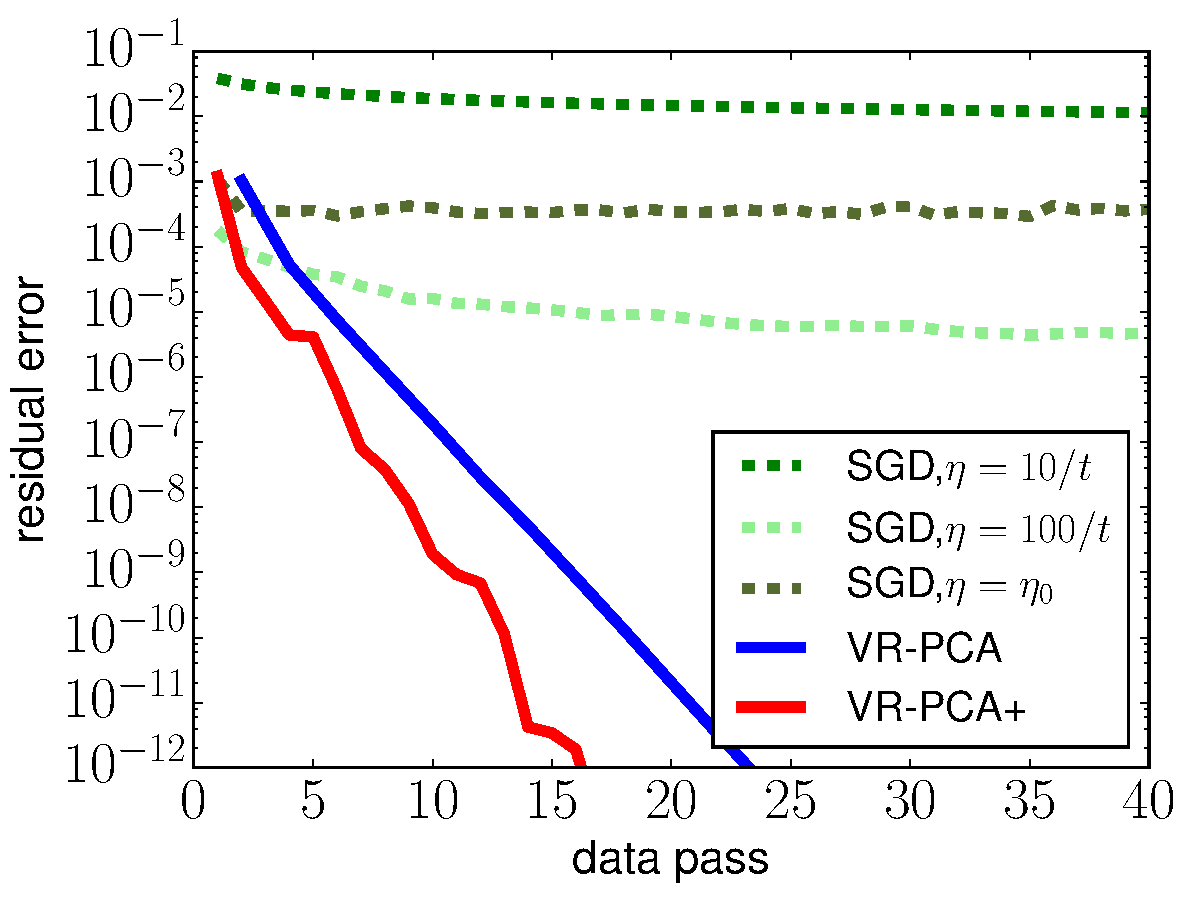
\includegraphics[width=0.495\columnwidth]{pca-4-mnist}\label{pca-4-mnist}}
\subfigure[mnist $k=6$]{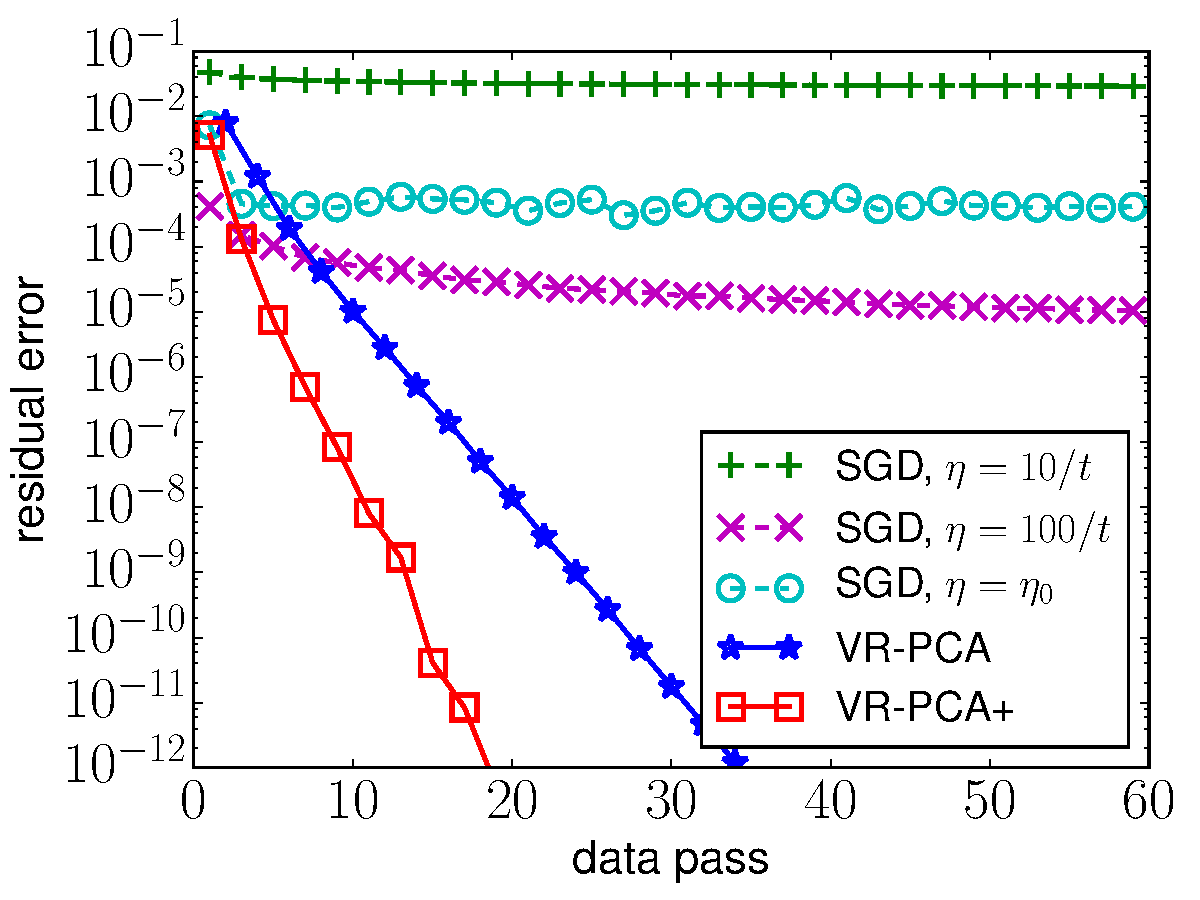
\includegraphics[width=0.495\columnwidth]{pca-6-mnist}\label{pca-6-mnist}}
%\subfigure[cifar10, $k=4$]{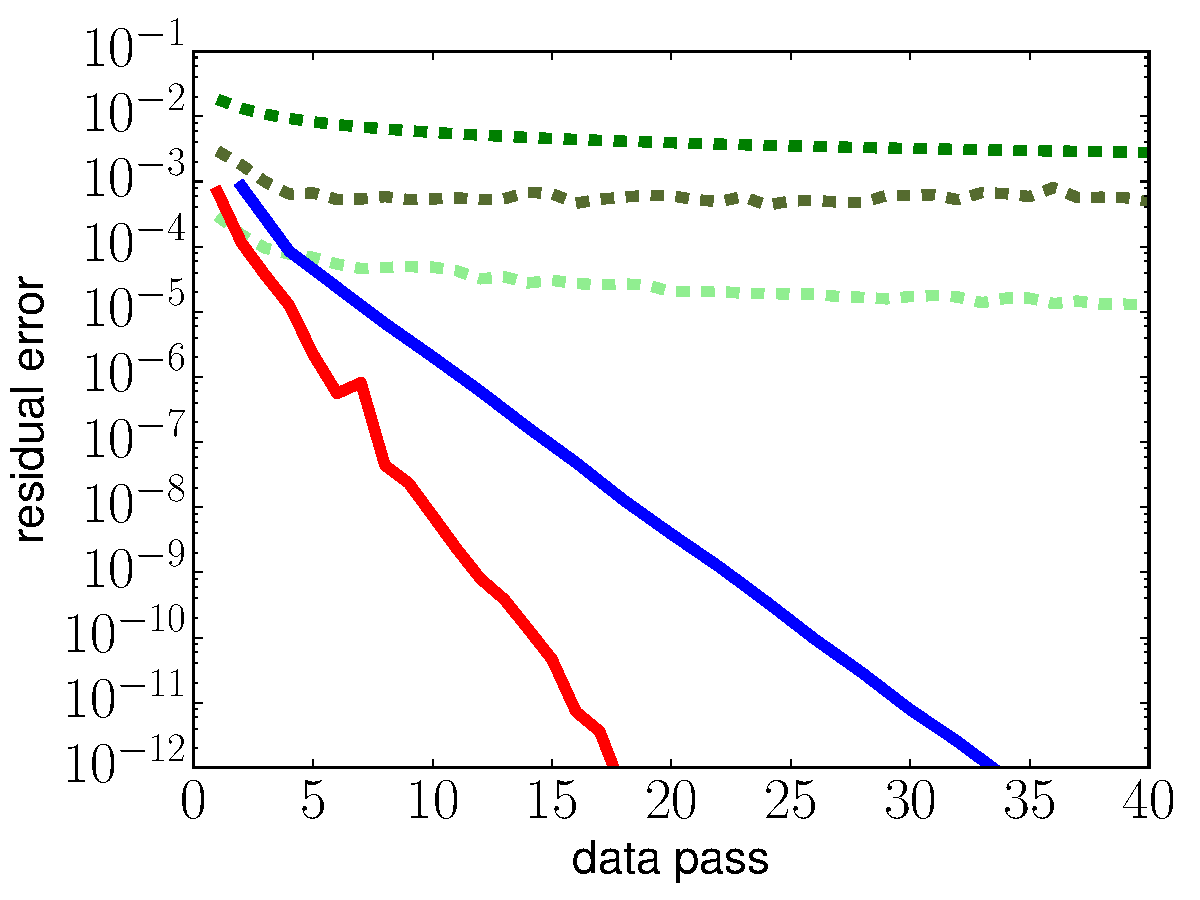
\includegraphics[width=0.495\columnwidth]{pca-4-cifar10}\label{pca-4-cifar10}}
\subfigure[cifar10 $k=6$]{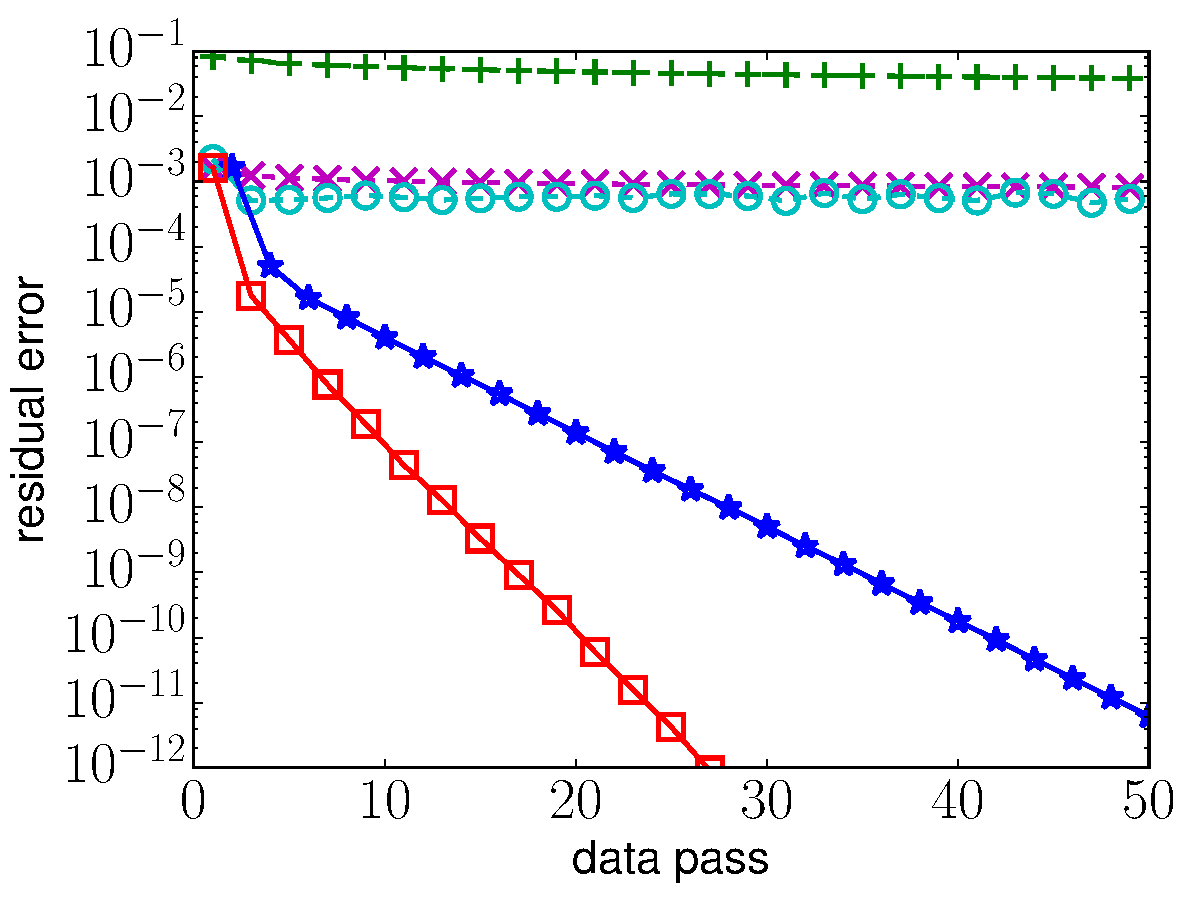
\includegraphics[width=0.495\columnwidth]{pca-6-cifar10}\label{pca-6-cifar10}}
%\subfigure[SVHN, $k=6$]{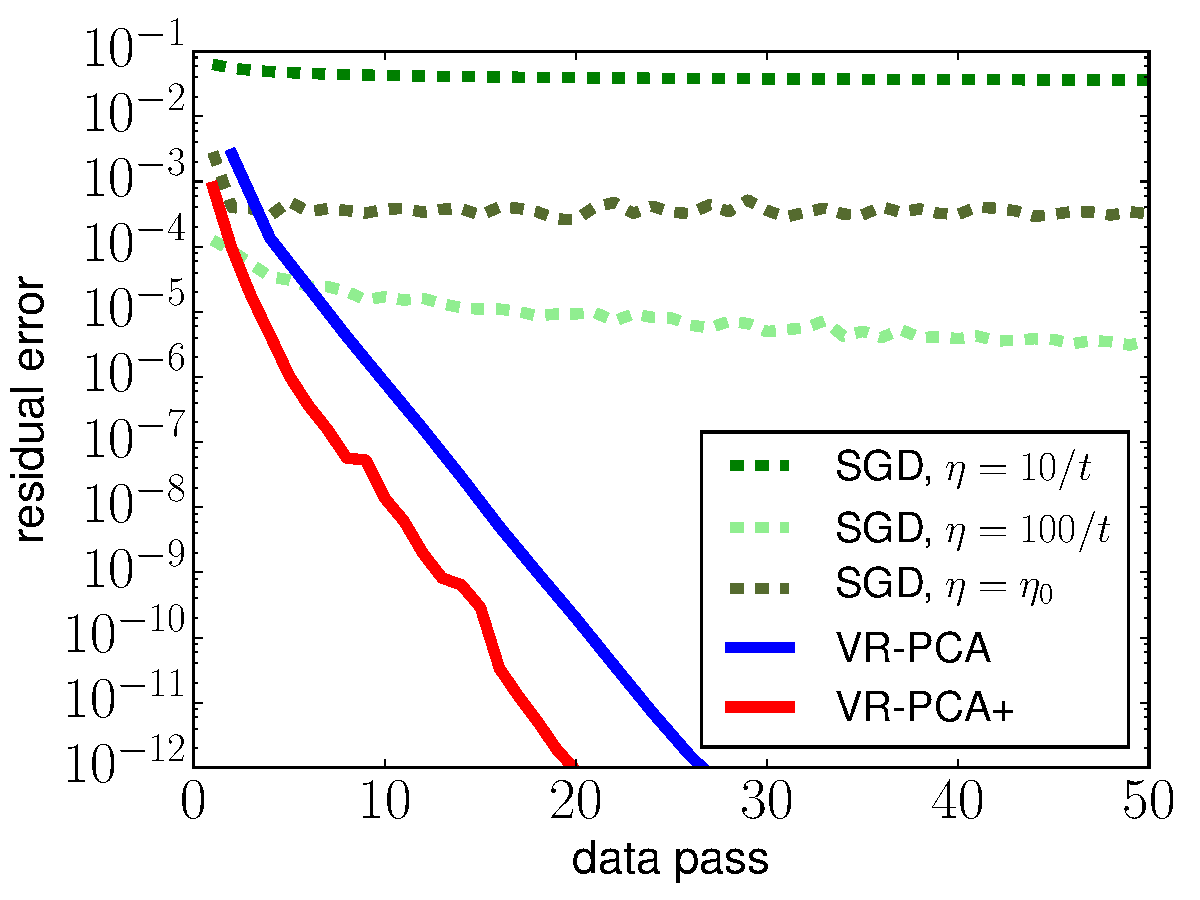
\includegraphics[width=0.5\columnwidth]{pca-6-SVHN}\label{pca-6-SVHN}}
%\subfigure[SVHN, $k=8$]{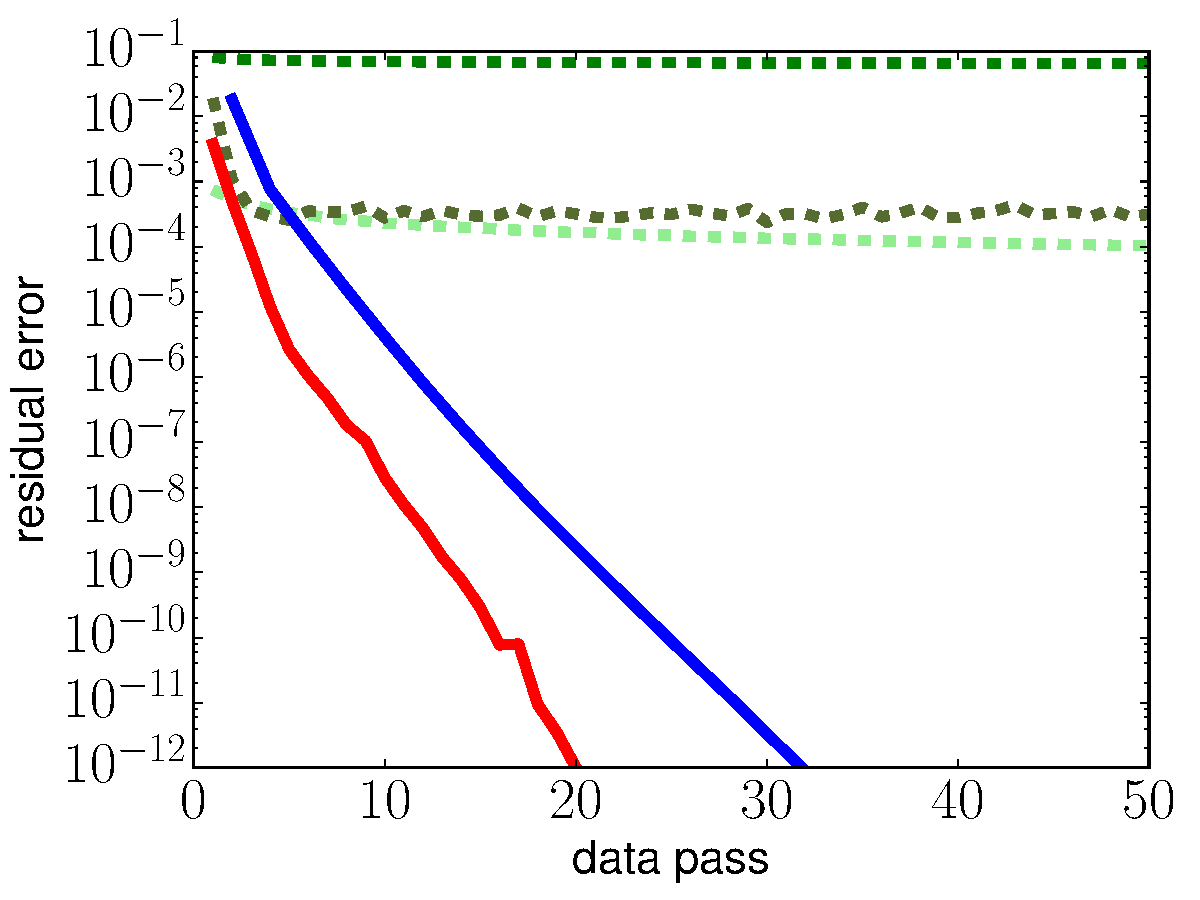
\includegraphics[width=0.495\columnwidth]{pca-8-SVHN}\label{pca-8-SVHN}}
%\subfigure[cifar100 $k=8$]{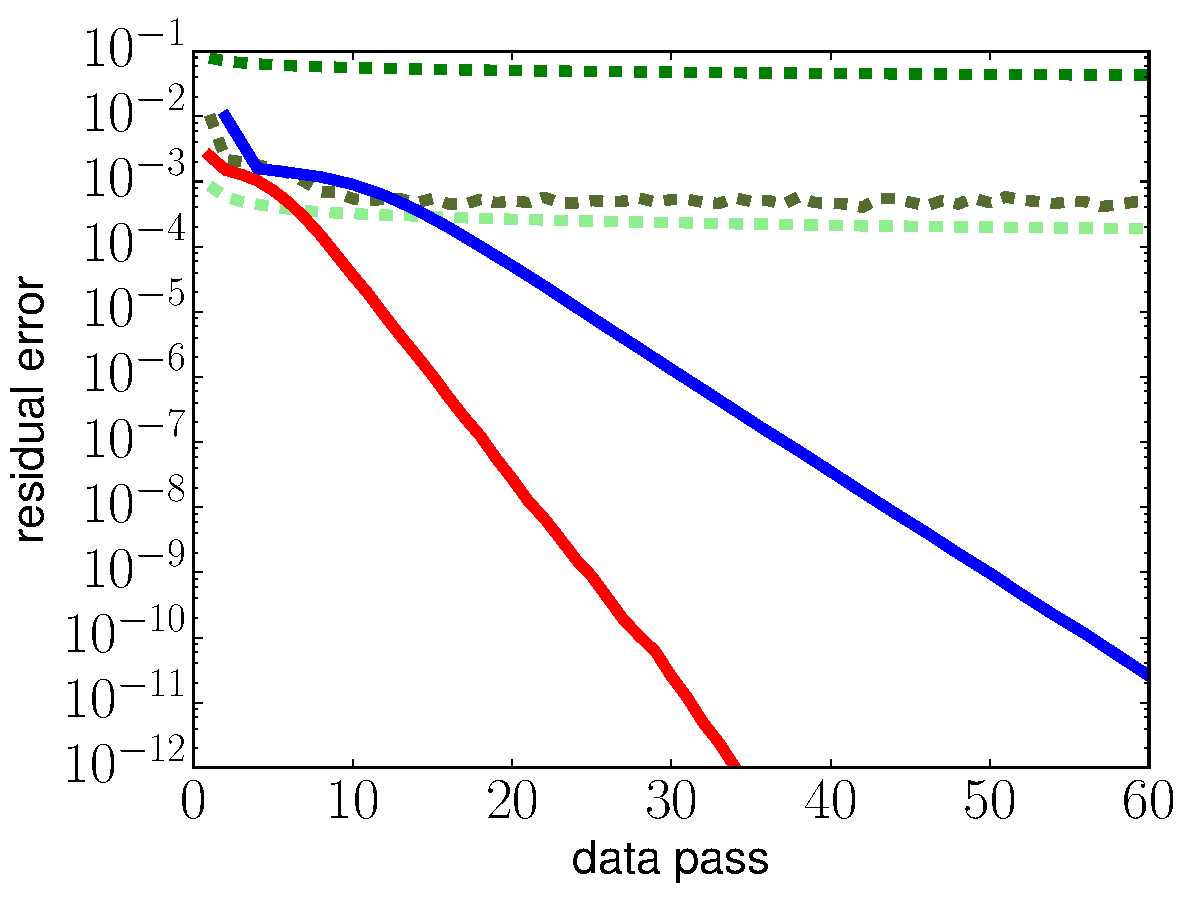
\includegraphics[width=0.495\columnwidth]{pca-8-cifar100}\label{pca-8-cifar100}}
%\subfigure[cifar100 $k=10$]{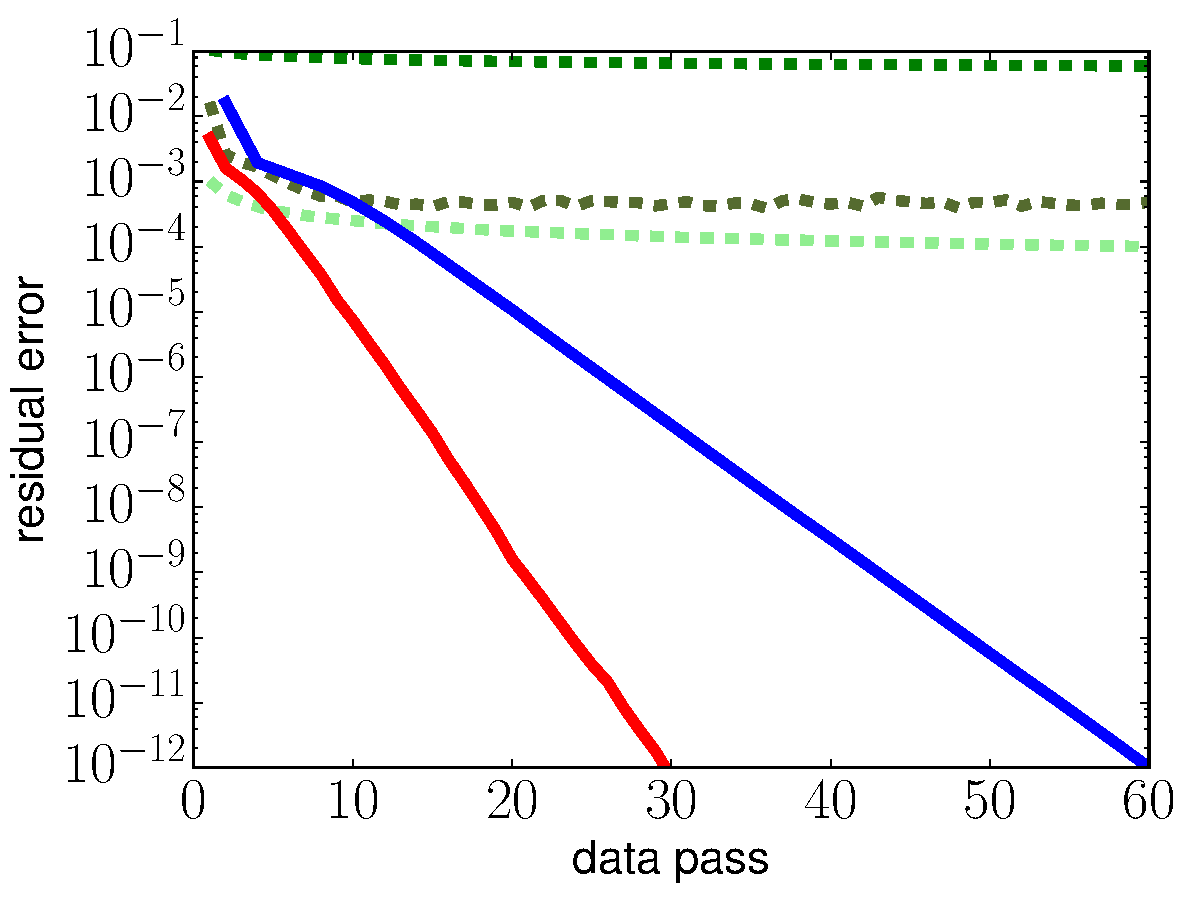
\includegraphics[width=0.5\columnwidth]{pca-10-cifar100}\label{pca-10-cifar100}}

%\caption{Generally, \textsc{aeSVRG} can automatically set an appropriate $m$ with different learning rates for the $l2$-regularized logistic regression on the dataset ijcnn1}
\caption{Generally, both VR-PCA and VR-PCA+ converge to a high precision and VR-PCA+ has a better performance.}
\label{pca}
\end{figure*}
 
 \begin{figure*}[ht]
\centering
%\subfigure[mnist, $k=4$]{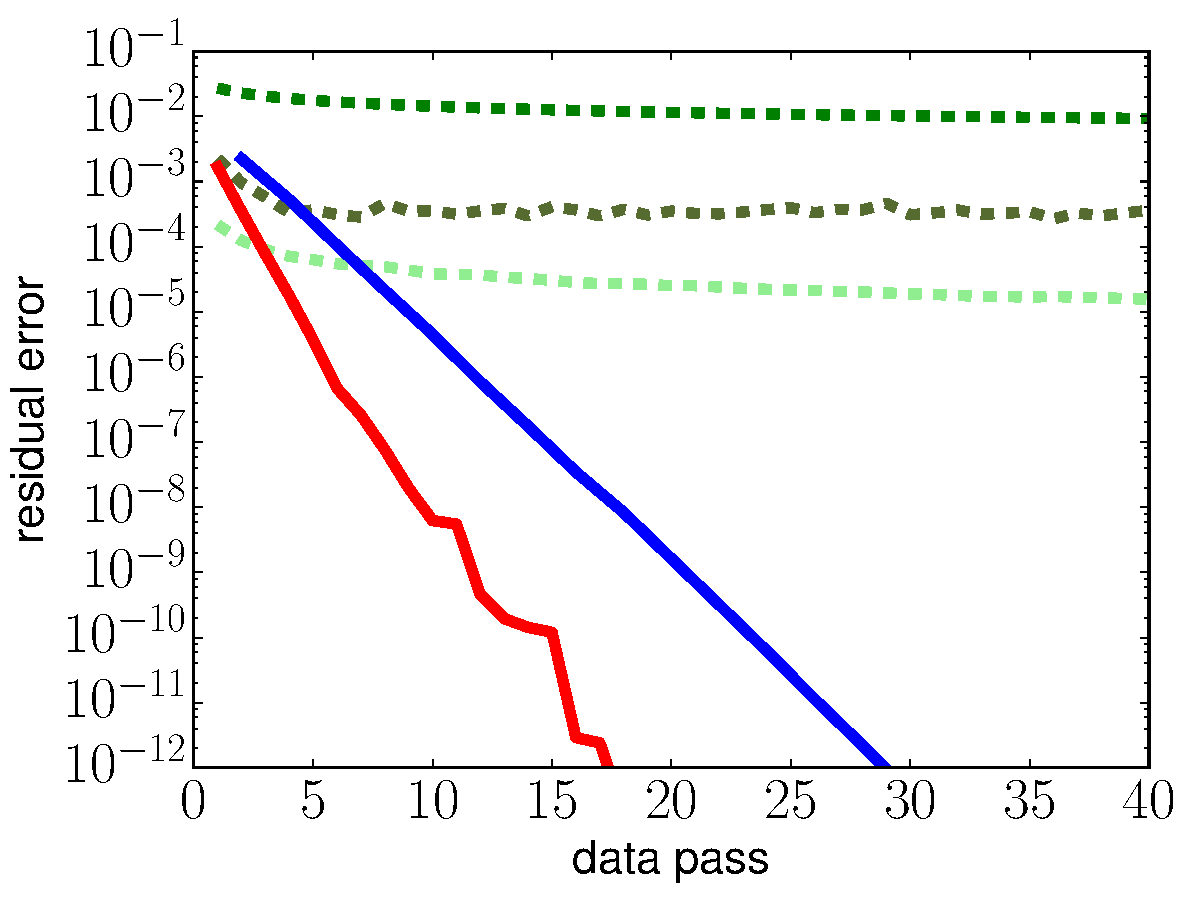
\includegraphics[width=0.5\columnwidth]{pls-4-mnist}\label{pls-4-mnist}}
%\subfigure[mnist $k=6$]{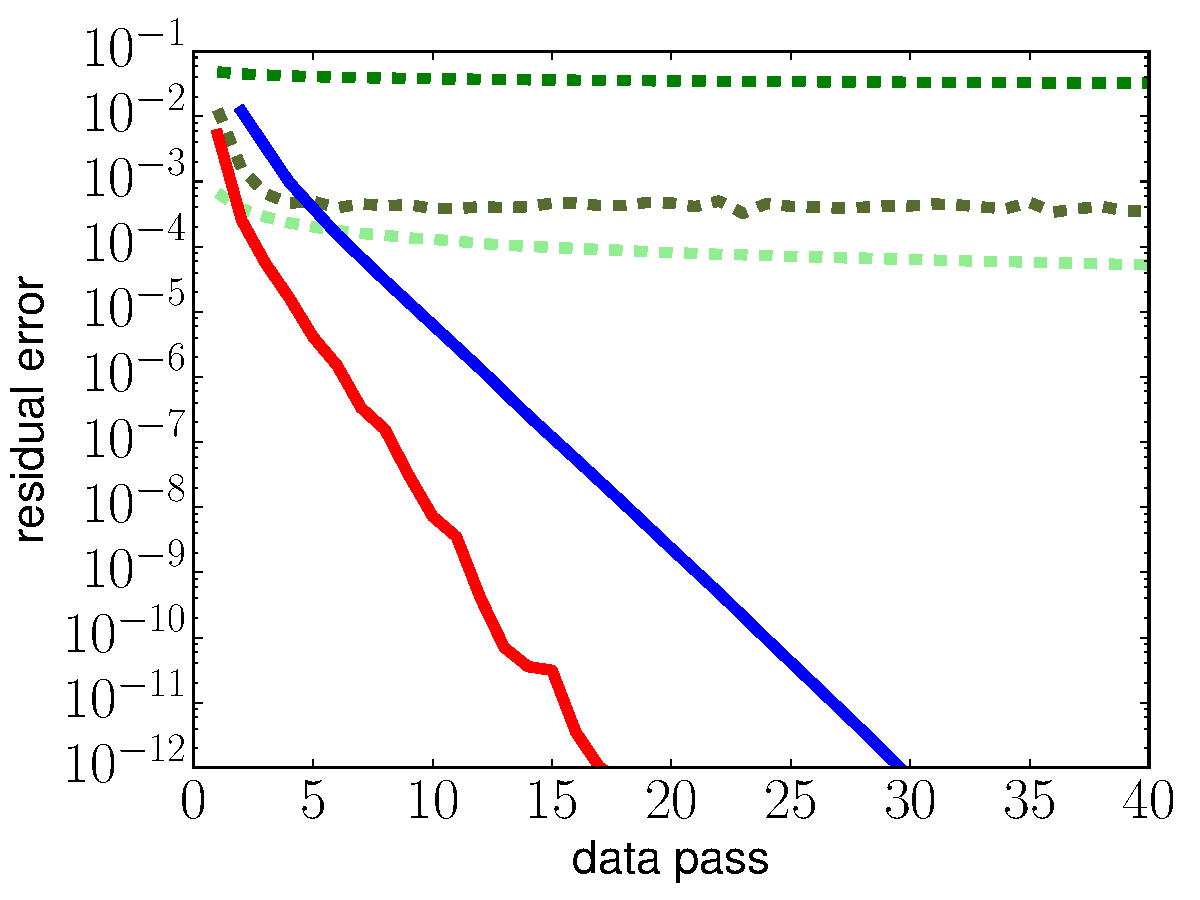
\includegraphics[width=0.495\columnwidth]{pls-6-mnist}\label{pls-6-mnist}}
%\subfigure[cifar10, $k=4$]{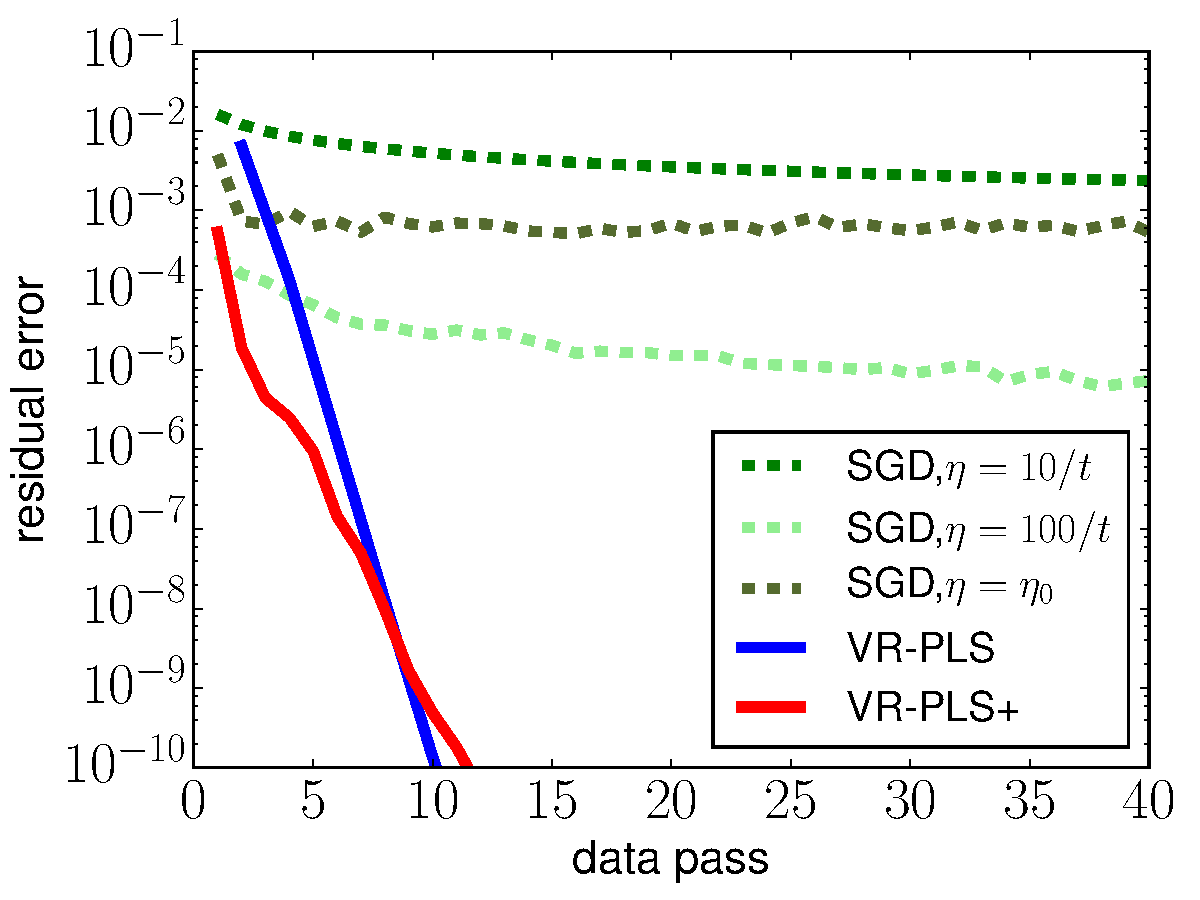
\includegraphics[width=0.5\columnwidth]{pls-4-cifar10}\label{pls-4-cifar10}}
%\subfigure[cifar10 $k=6$]{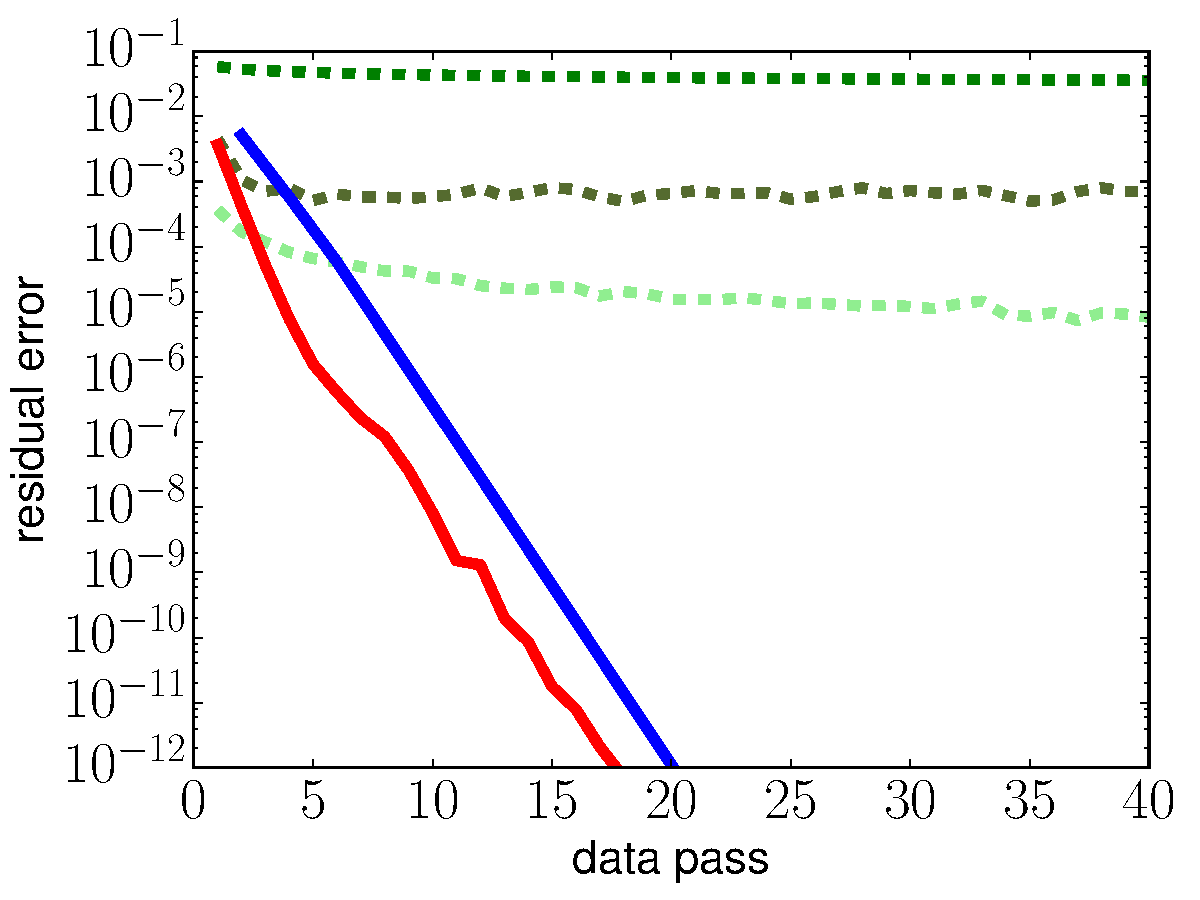
\includegraphics[width=0.495\columnwidth]{pls-6-cifar10}\label{pls-6-cifar10}}
%\subfigure[SVHN, $k=6$]{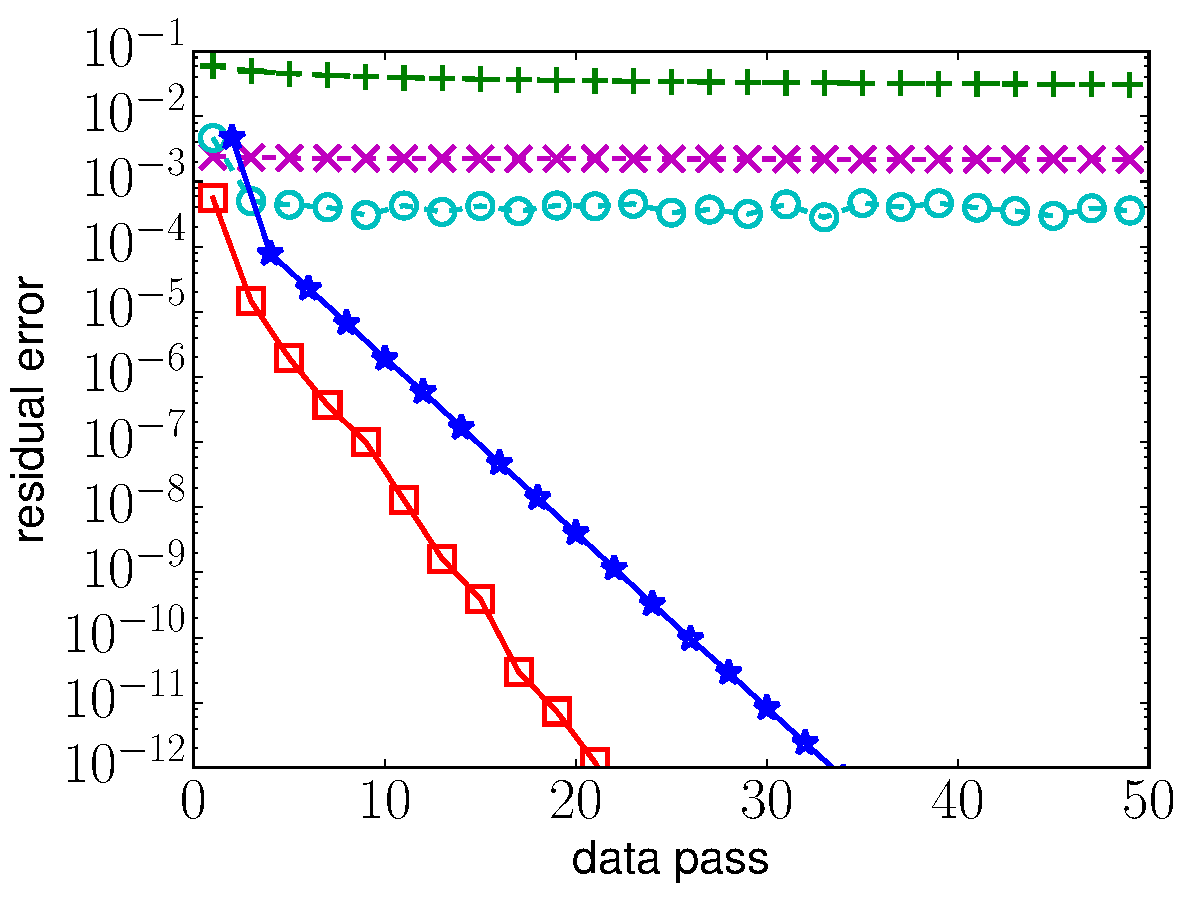
\includegraphics[width=0.5\columnwidth]{pls-6-SVHN}\label{pls-6-SVHN}}
\subfigure[SVHN, $k=8$]{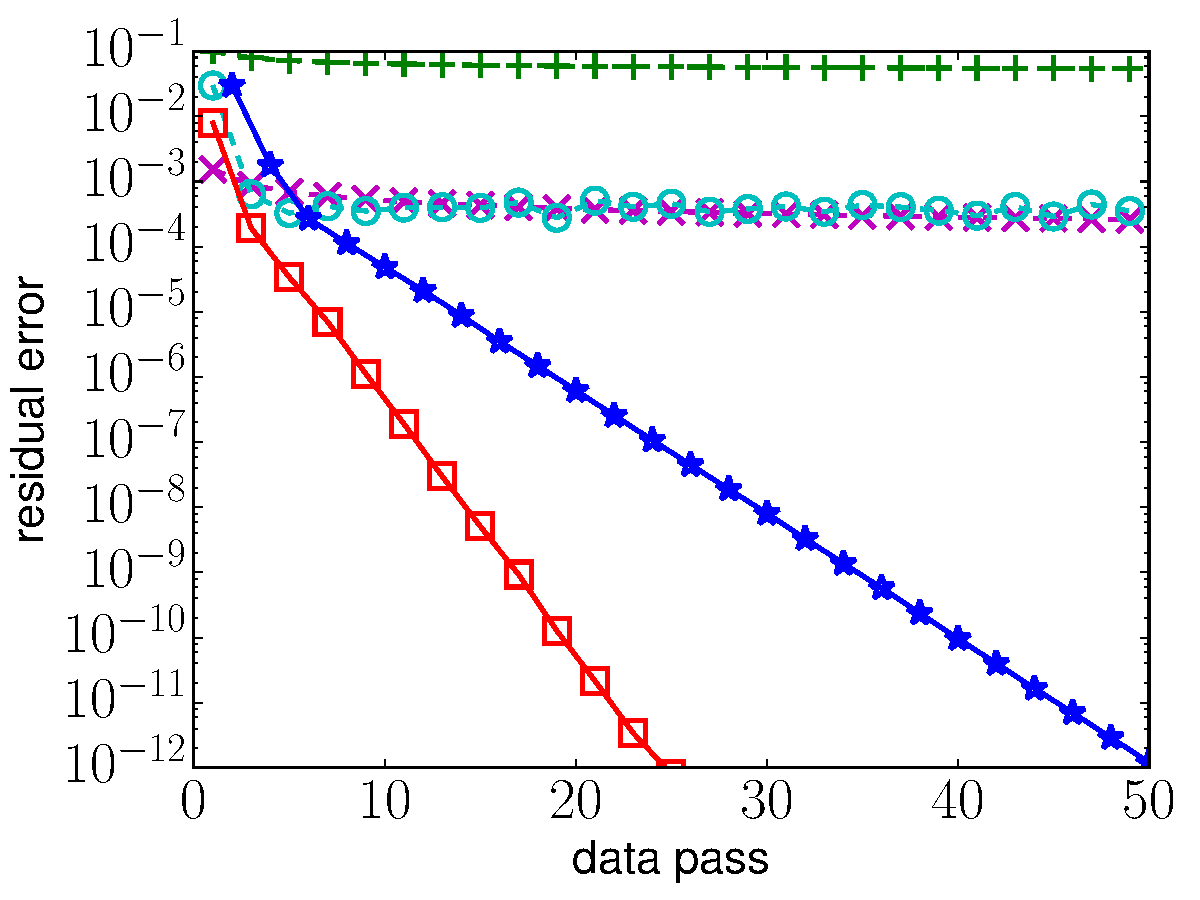
\includegraphics[width=0.495\columnwidth]{pls-8-SVHN}\label{pls-8-SVHN}}
\subfigure[cifar100 $k=8$]{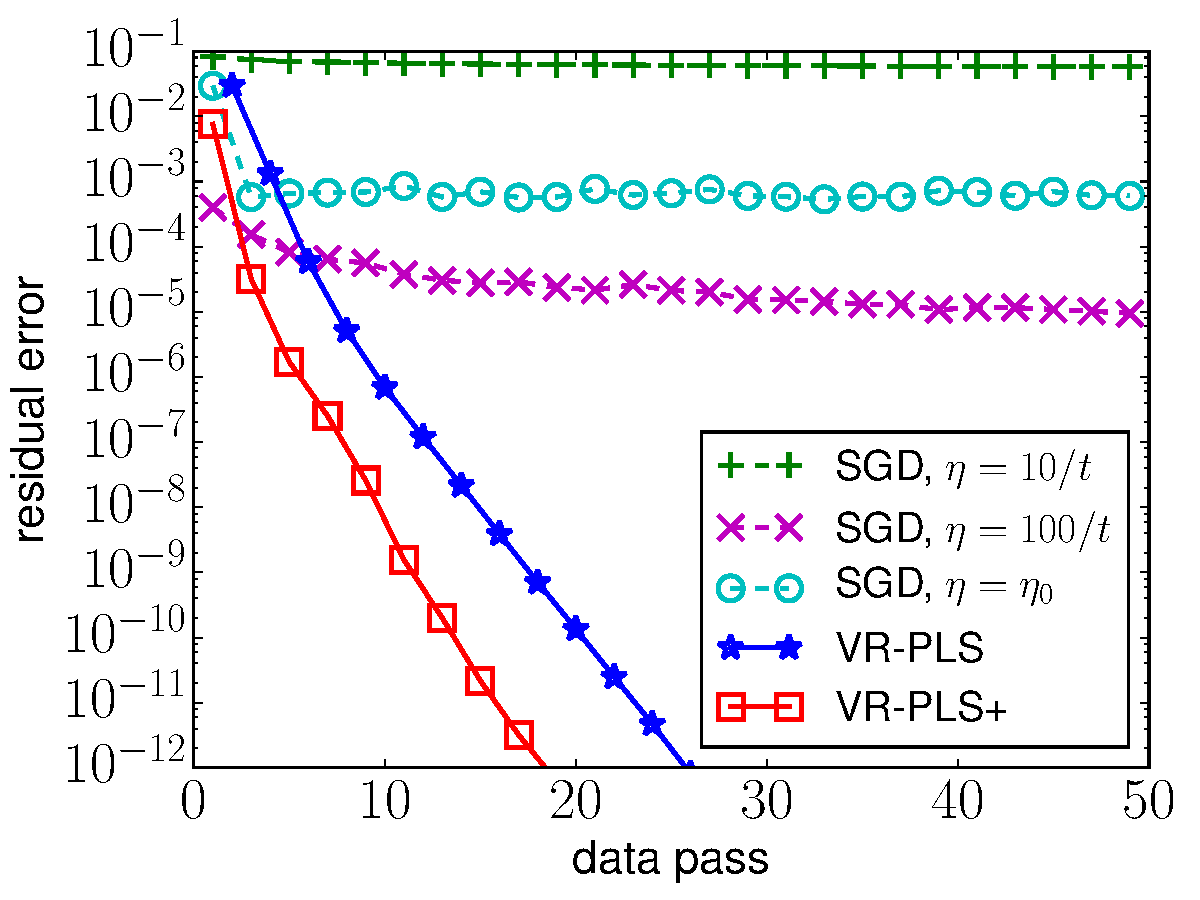
\includegraphics[width=0.495\columnwidth]{pls-8-cifar100}\label{pls-8-cifar100}}
%\subfigure[cifar100 $k=10$]{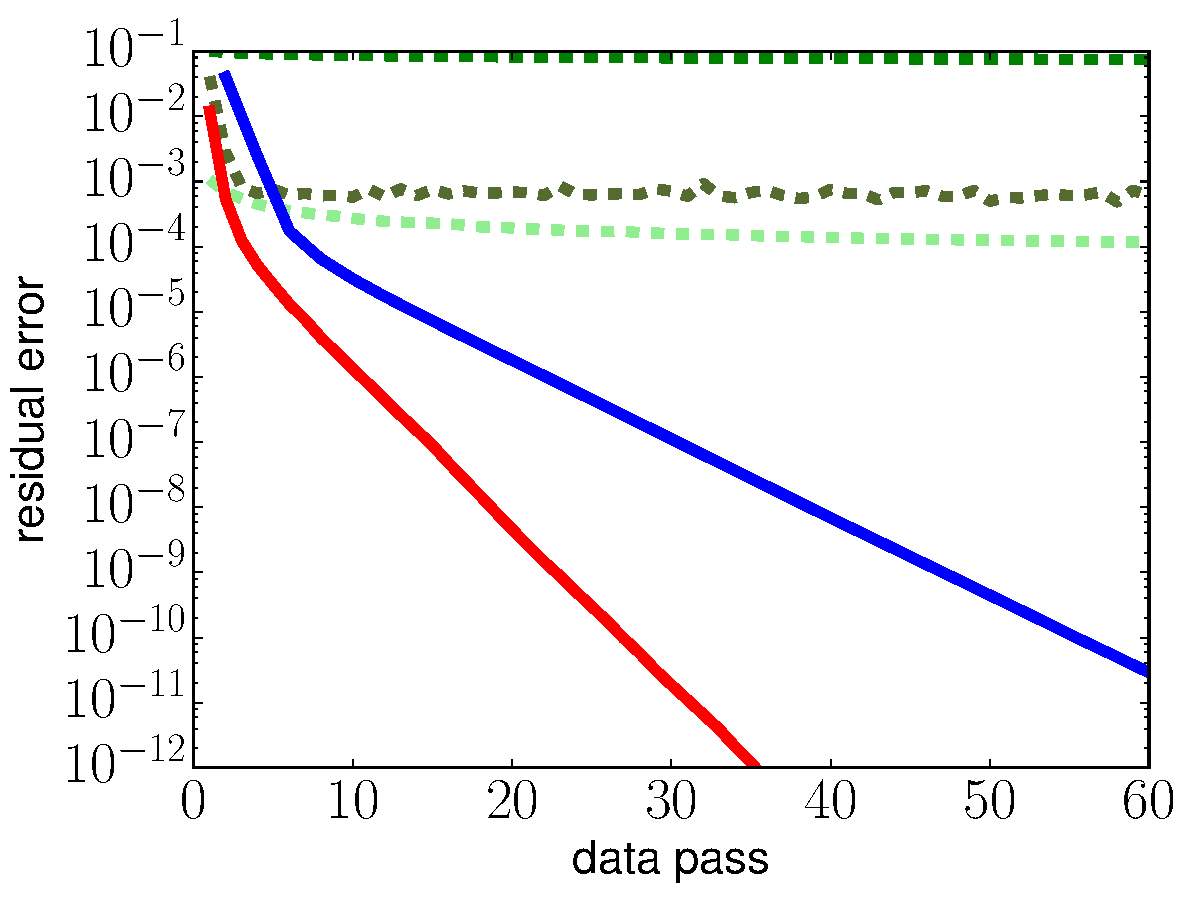
\includegraphics[width=0.5\columnwidth]{pls-10-cifar100}\label{pls-10-cifar100}}

%\caption{Generally, \textsc{aeSVRG} can automatically set an appropriate $m$ with different learning rates for the $l2$-regularized logistic regression on the dataset ijcnn1}
\caption{Generally, both VR-PLS and VR-PLS+ converge to a high precision and VR-PLS+ has a better performance in most cases.}
\label{pls}
\end{figure*}
 

 
 
 \begin{figure*}[ht]
\centering
\subfigure[mnist, $k=4$, pca]{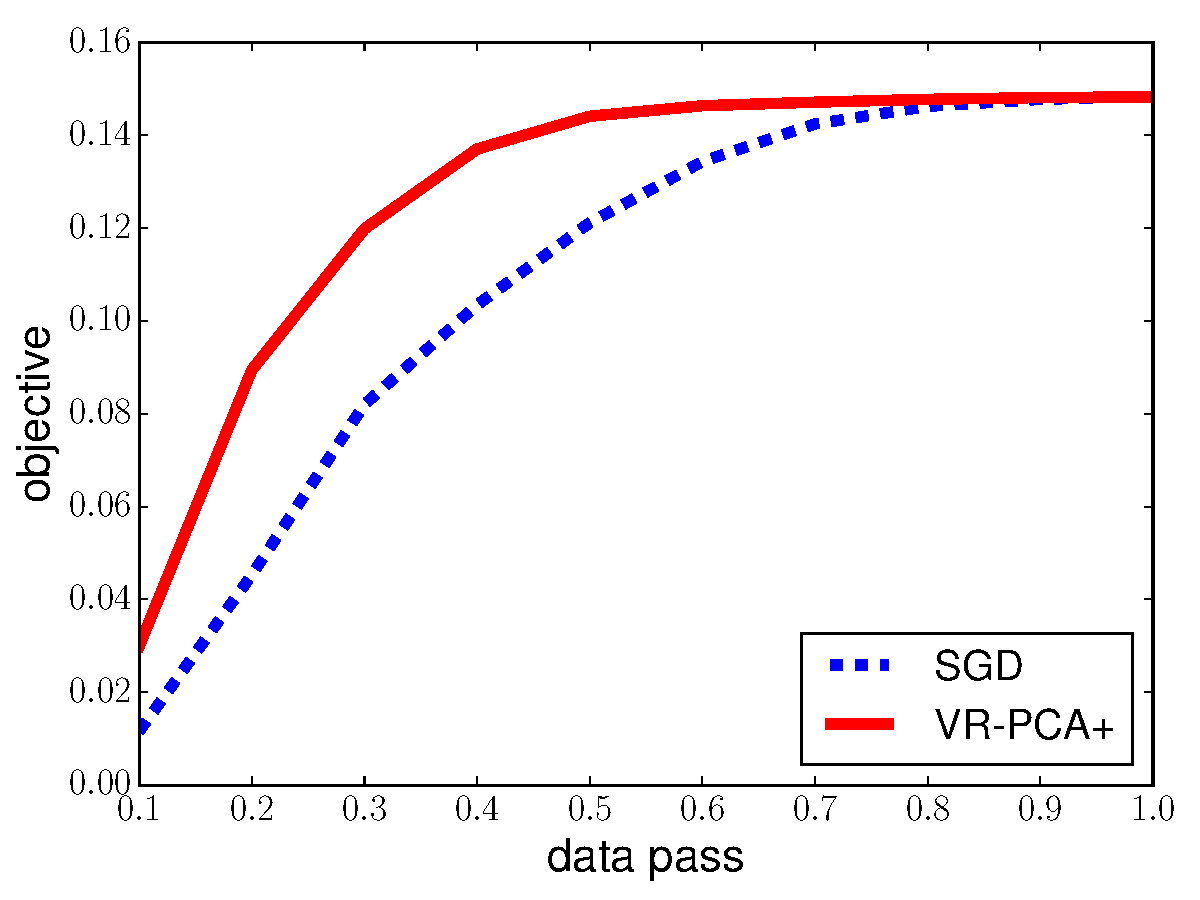
\includegraphics[width=0.495\columnwidth]{one-pca-4-mnist}\label{o-pca-4-mnist}}
%\subfigure[mnist $k=6$, pca]{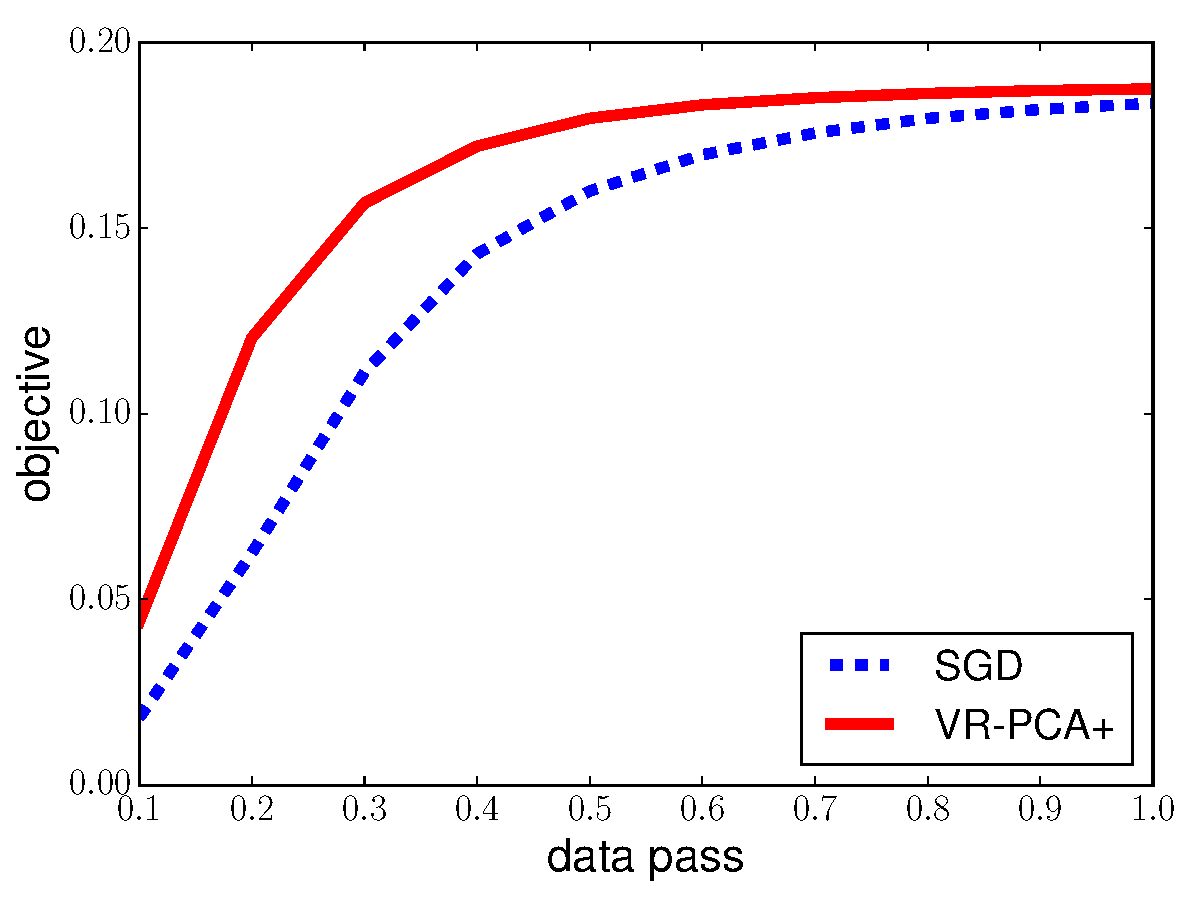
\includegraphics[width=0.495\columnwidth]{one-pca-6-mnist}\label{o-pca-6-mnist}}
%\subfigure[cifar10, $k=4$, pls]{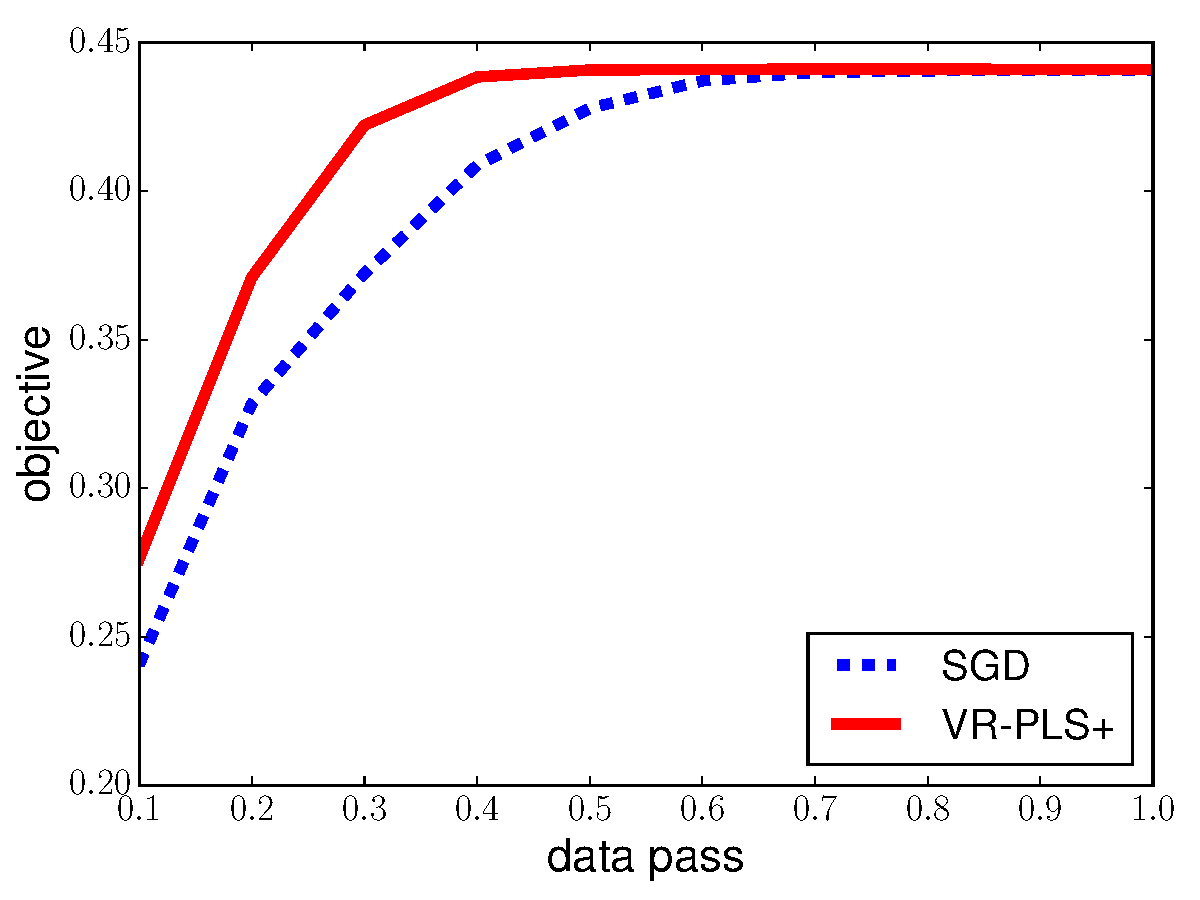
\includegraphics[width=0.495\columnwidth]{one-pls-4-cifar10}\label{o-pls-4-cifar10}}
\subfigure[cifar10 $k=6$, pls]{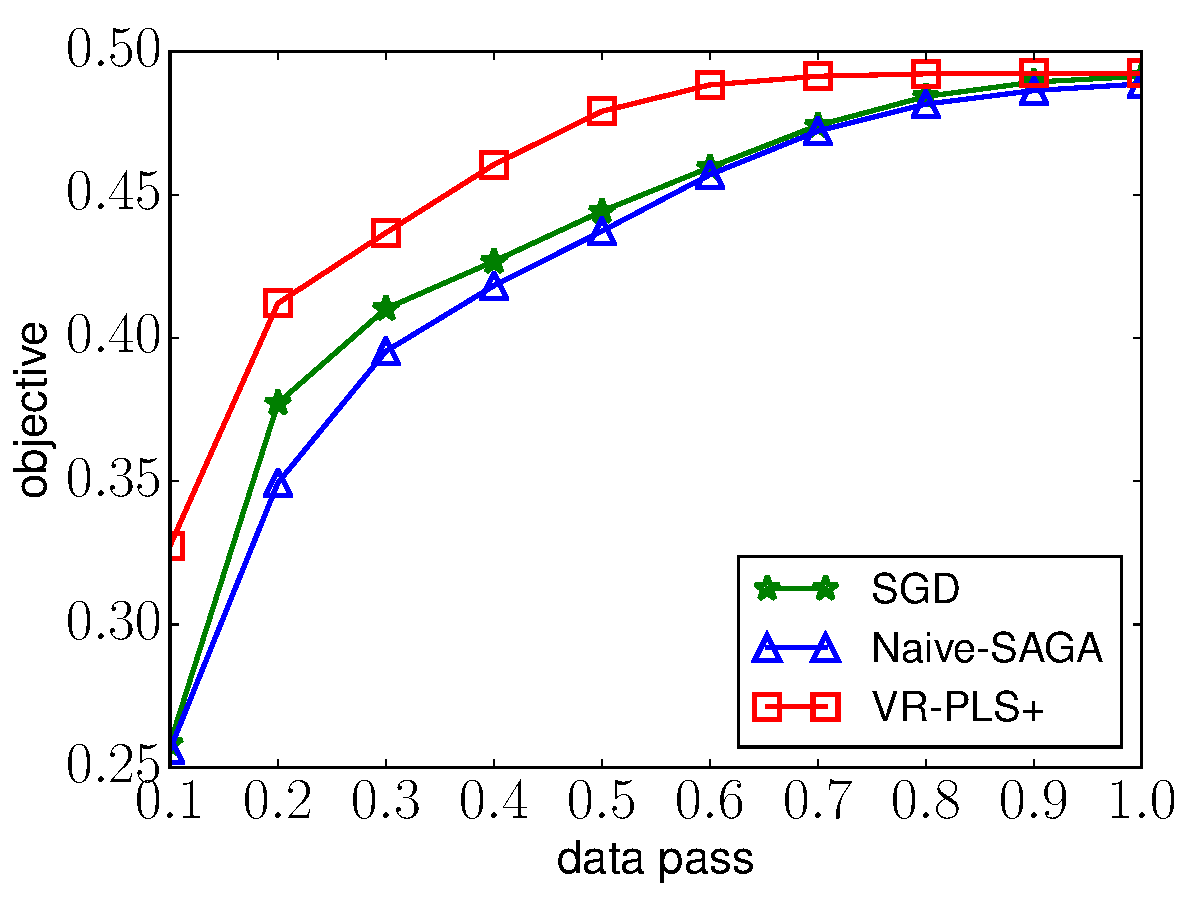
\includegraphics[width=0.495\columnwidth]{one-pls-6-cifar10}\label{o-pls-6-cifar10}}
\caption{VR-PCA(PLS)+ performs better than SGD and Naive-SAGA in the first data pass.}
\label{one pass}
\end{figure*}
 
 \subsection{Experiments for high-precision requirement}
 In this section we demonstrate the effectiveness and efficiency of our proposed algorithms. The evaluation criterion is the progress made on the objective as a function of iteration number, which is suitable for evaluating gradient optimization algorithms. 
 For comparison, we also implemented the SGD algorithm and SVRG-based algorithms, i.e., VR-PCA and VR-PLS. Note that VR-PLS is naturally extended from VR-PCA, just replacing the update rule.
 We did not implement other sophisticated iterative algorithms mentioned in Section \ref{introduction} for the same reason with \citep{Shamir2015A}, as they are not directly comparable to the stochastic gradient algorithms due to inherent complexity per iteration and considerable memory requirement.
  The algorithms compared were initialized from the same random matrices. The results are displayed in Figure \ref{pca} and Figure \ref{pls}.
  In all figures, the x-axis represents the number of effective data passes,
  % (assuming 2 per epoch for VR-PCA and VR-PLS, 1 per epoch for VR-PCA+ and VR-PLS+)
  and the y-axis represent the residual, i.e., $tr(\hat{W}^{\top}X^{\top}X\hat{W}) - tr(W^{\top}X^{\top}XW)$ for PCA and $tr(\hat{U}^{\top}X^{\top}Y\hat{V}) - tr(U^{\top}X^{\top}YV)$ for PLS. Note the $X$,$Y$ are the data matrices, $\hat{W}$, $\hat{U}$, $\hat{V}$ are the optimal parameter matrices obtained by SVD, W, U, V are the matrices obtained so far. 
 From the figures we see that for different datasets and $k$, SGD algorithms appears to have a sub-linear convergence rate and fail to achieve a high-precision result, no matter which step strategy is applied.
In contrast, both VR-PCA(PLS) and VR-PCA(PLS)+ rapidly converge to an accuracy higher than $10^{-10}$, the main reason is that they have much lower variance than naive SGD algorithm. Besides, we  find the VR-PCA(PLS)+ have a better performance than VR-PCA(PLS). It is not surprising since the SAGA-based algorithms do not require to compute the batch-gradient occasionally, which is time-consuming.
 
 \subsection{Experiments with limited time overhead}
 In this part we limit the computational cost within one data pass. Since VR-PCA(PLS) do not optimize the objective function in the first data pass, they were not experimented. Hence we only compare the VR-PCA(PLS)+ with SGD algorithm. In particular, apart from our proposed VR-PCA(PLS)+, we also implement another variant called Naive-SAGA, which abandons the preparation step directly without modification. The goal is to demonstrate the superiority of our proposed sample strategy and new update rule of $\tilde{\mu}$.
 We set the learning rate as $\eta_0$ for all experiments.
 The results are illustrated in figure \ref{one pass}.  Note that the x-axis still represents the number of data passes while the y-axis denotes the value of objective function. As we can see in figure \ref{one pass}, VR-PCA(PLS)+ always has the best performance, the main reason is that the variance reduced stochastic gradient of VR-PCA(PLS)+ is the combination of a stochastic gradient and a stale mini-batch gradient, which has a smaller variance.

 


\section{Conclusion and Future Works}
\label{discussion}
Deterministic optimization algorithms for PCA and PLS suffer from unbearable computation cost in large-scale application, while stochastic algorithm is prohibitive from a high-accuracy solution. Thus it is natural to apply the variance reduced stochastic method to solve PCA and PLS. In this paper, we propose the novel
SAGA-based algorithms, which perform better than SVRG-based algorithms and apply to time limited conditions. 
Although we have not rigorously conducted convergence analysis on the proposed algorithms, all of them prove to be experimentally efficient.
We leave the following future works: (1) Prove the convergence of proposed algorithms theoretically. (2) Research the asynchronous variants of VR-PCA+ and VR-PLS+. (3) Explore other constrained objective functions which can be optimized through stochastic power methods and its variance reduced variants.



\section*{Acknowledgment}







%\bibliographystyle{plain}
\bibliographystyle{unsrt}
\bibliography{reference}




\end{document}
